% Options for packages loaded elsewhere
\PassOptionsToPackage{unicode}{hyperref}
\PassOptionsToPackage{hyphens}{url}
%
\documentclass[
]{book}
\usepackage{amsmath,amssymb}
\usepackage{lmodern}
\usepackage{iftex}
\ifPDFTeX
  \usepackage[T1]{fontenc}
  \usepackage[utf8]{inputenc}
  \usepackage{textcomp} % provide euro and other symbols
\else % if luatex or xetex
  \usepackage{unicode-math}
  \defaultfontfeatures{Scale=MatchLowercase}
  \defaultfontfeatures[\rmfamily]{Ligatures=TeX,Scale=1}
\fi
% Use upquote if available, for straight quotes in verbatim environments
\IfFileExists{upquote.sty}{\usepackage{upquote}}{}
\IfFileExists{microtype.sty}{% use microtype if available
  \usepackage[]{microtype}
  \UseMicrotypeSet[protrusion]{basicmath} % disable protrusion for tt fonts
}{}
\makeatletter
\@ifundefined{KOMAClassName}{% if non-KOMA class
  \IfFileExists{parskip.sty}{%
    \usepackage{parskip}
  }{% else
    \setlength{\parindent}{0pt}
    \setlength{\parskip}{6pt plus 2pt minus 1pt}}
}{% if KOMA class
  \KOMAoptions{parskip=half}}
\makeatother
\usepackage{xcolor}
\IfFileExists{xurl.sty}{\usepackage{xurl}}{} % add URL line breaks if available
\IfFileExists{bookmark.sty}{\usepackage{bookmark}}{\usepackage{hyperref}}
\hypersetup{
  pdftitle={Reloc-Age},
  hidelinks,
  pdfcreator={LaTeX via pandoc}}
\urlstyle{same} % disable monospaced font for URLs
\usepackage{longtable,booktabs,array}
\usepackage{calc} % for calculating minipage widths
% Correct order of tables after \paragraph or \subparagraph
\usepackage{etoolbox}
\makeatletter
\patchcmd\longtable{\par}{\if@noskipsec\mbox{}\fi\par}{}{}
\makeatother
% Allow footnotes in longtable head/foot
\IfFileExists{footnotehyper.sty}{\usepackage{footnotehyper}}{\usepackage{footnote}}
\makesavenoteenv{longtable}
\usepackage{graphicx}
\makeatletter
\def\maxwidth{\ifdim\Gin@nat@width>\linewidth\linewidth\else\Gin@nat@width\fi}
\def\maxheight{\ifdim\Gin@nat@height>\textheight\textheight\else\Gin@nat@height\fi}
\makeatother
% Scale images if necessary, so that they will not overflow the page
% margins by default, and it is still possible to overwrite the defaults
% using explicit options in \includegraphics[width, height, ...]{}
\setkeys{Gin}{width=\maxwidth,height=\maxheight,keepaspectratio}
% Set default figure placement to htbp
\makeatletter
\def\fps@figure{htbp}
\makeatother
\setlength{\emergencystretch}{3em} % prevent overfull lines
\providecommand{\tightlist}{%
  \setlength{\itemsep}{0pt}\setlength{\parskip}{0pt}}
\setcounter{secnumdepth}{5}
\usepackage{booktabs}
\ifLuaTeX
  \usepackage{selnolig}  % disable illegal ligatures
\fi
\usepackage[]{natbib}
\bibliographystyle{plainnat}

\title{Reloc-Age}
\author{}
\date{\vspace{-2.5em}}

\begin{document}
\maketitle

{
\setcounter{tocdepth}{1}
\tableofcontents
}
\hypertarget{about}{%
\chapter{About}\label{about}}

RELOC-AGE: How Do Housing Choices and Relocation Matter for Active and Healthy Ageing?

To generate novel and significant knowledge on housing choices and relocation as related to active and healthy ageing,
the objectives of this multistage mixed methods participatory project are to:

\begin{itemize}
\tightlist
\item
  Study housing choices, relocation and health patterns in the Swedish population aged 55+ (Register
  RELOC-AGE).
\item
  Study housing choices and relocation and examine the effects on active and healthy ageing among people
  aged 55+ considering relocation (Prospective RELOC-AGE).
\item
  Complete the development of a novel housing counselling intervention and a subsequent pilot study
  (Intervention RELOC-AGE).
\item
  Contribute to theory development (Theory RELOC-AGE).
\end{itemize}

\hypertarget{research-questions}{%
\chapter{Research questions}\label{research-questions}}

\begin{enumerate}
\def\labelenumi{\arabic{enumi}.}
\tightlist
\item
  What are the trends over time and by age when it comes to housing types and tenures?
\item
  How do housing aspects and relocations affect future health outcomes?
\end{enumerate}

\begin{itemize}
\tightlist
\item
  How are these patterns affected by age, sex, civil status, country of origin, adverse health
  events, loss of a partner, socio-economic and neighbourhood characteristics?
\item
  Given equal propensity of relocation based on baseline demographic, socio-economic and
  health characteristics, how do specific housing decisions affect future health outcomes?
\end{itemize}

\begin{enumerate}
\def\labelenumi{\arabic{enumi}.}
\setcounter{enumi}{2}
\tightlist
\item
  What are the effects of adverse health events on housing choices and relocation patterns?
\end{enumerate}

\begin{itemize}
\tightlist
\item
  What are the short- and long-term effects?
\item
  How do these effects differ between men and women, across different disease and/or disability profiles, civil status, country of origin and socio-economic status?
\end{itemize}

\begin{enumerate}
\def\labelenumi{\arabic{enumi}.}
\setcounter{enumi}{3}
\tightlist
\item
  What aspects of housing and health predict:
\end{enumerate}

\begin{itemize}
\tightlist
\item
  relocation to different housing options in the ordinary housing stock
\item
  relocation to residential care facilities
\item
  remaining in the present dwelling?
\end{itemize}

\begin{enumerate}
\def\labelenumi{\arabic{enumi}.}
\setcounter{enumi}{4}
\tightlist
\item
  How is the complex interaction between objective and perceived aspects of housing and social aspects associated with active and healthy ageing, and what are the characteristics and trajectories of such dynamics?
\item
  What housing attributes do older adults considering relocation find important, and to what extent, when making their decisions on housing preferences?
\item
  How do older adults considering relocation reason regarding:
\end{enumerate}

\begin{itemize}
\tightlist
\item
  different housing options and
\item
  motives for considering and effectuating relocation, and
\item
  to what extent are their motives fulfilled?
\end{itemize}

\begin{enumerate}
\def\labelenumi{\arabic{enumi}.}
\setcounter{enumi}{7}
\tightlist
\item
  Is the newly developed housing counselling intervention usable, feasible and acceptable for the Swedish municipality context, and what are the pros and cons of different delivery formats?
\item
  Which outcomes should be used to investigate the effectiveness of housing counselling, and what are
\end{enumerate}

\begin{itemize}
\tightlist
\item
  the responsiveness and,
\item
  the intervention effects on the selected primary and secondary outcomes, as indicated by the results of the pilot study?
\end{itemize}

\begin{enumerate}
\def\labelenumi{\arabic{enumi}.}
\setcounter{enumi}{9}
\tightlist
\item
  What are the main concepts and pathways of a theory on housing choices, relocation and active ageing?
\end{enumerate}

\hypertarget{intro}{%
\chapter{Introduction}\label{intro}}

Here is the introduction and outline of the document.

Here is some test text. I am typing, I am typing, I am not a robot.

\hypertarget{description-of-data-sets}{%
\chapter{Description of data sets}\label{description-of-data-sets}}

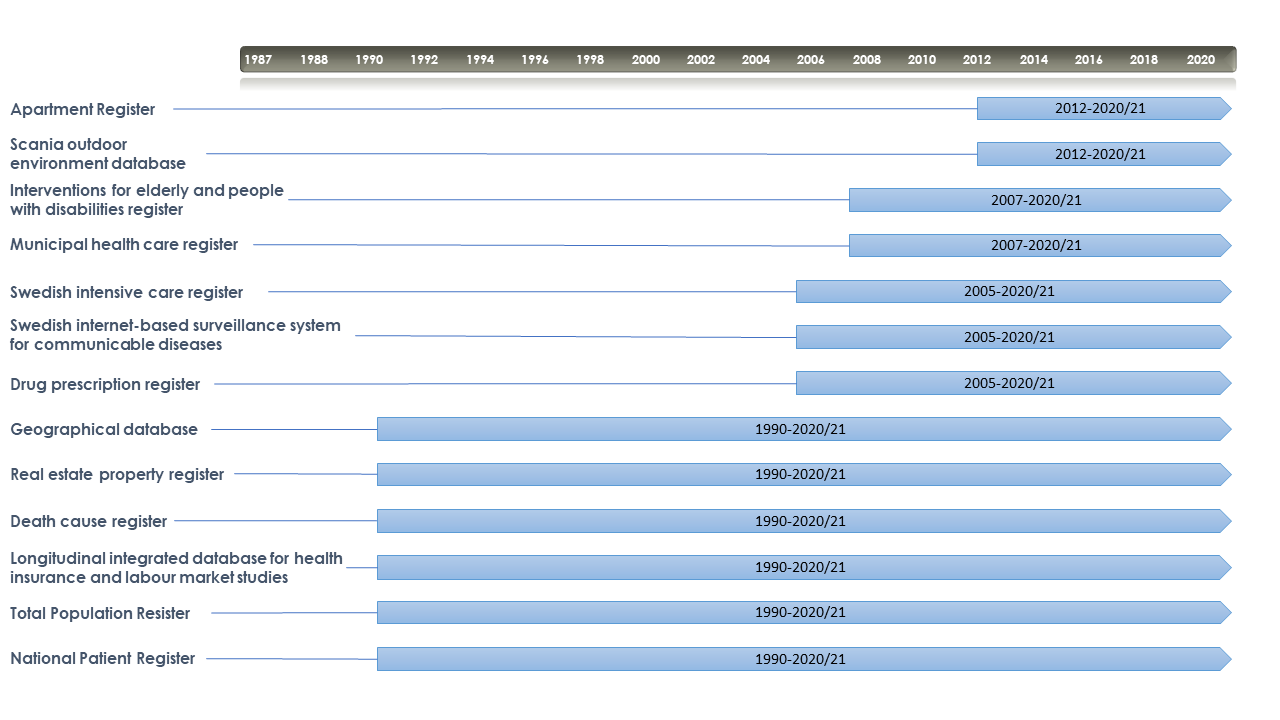
\includegraphics[width=17.78in]{output/figures/registers_timeline}

\hypertarget{data-cleaning-and-joining-of-data}{%
\section{Data cleaning and joining of data}\label{data-cleaning-and-joining-of-data}}

As illustrated above, the Reloc-Age data set is comprised of data from several registers and sources. In order to arrive at the final data set, a number of data cleaning actions, multiple joins, and many quality control steps have been taken to insure reliable analysis and data integrity. This section details steps taken.

\hypertarget{scb-data}{%
\subsection{SCB data}\label{scb-data}}

A significant amount of data from the registrars originates from Statistics Sweden (SCB). This data is delivered in text format (file extension .txt), and is partitioned, for the most part, into individual files separated by both year and data set.

With data covering about 3 million individuals over a period of decades and consisting of multitude of variables contained in hundreds of very large files, the computational effort to complete these joins are very time intensive, often taking hours for each merge, with progress occasionally hindered by computational restrictions and small errors which arise in the data cleaning process. With this in mind, detailed documentation, contained both here and alongside code used in the data cleaning, is prioritized to reduce any need to repeat these time-intensive processes.

\begin{itemize}
\tightlist
\item
  Raw data files are organized into folder structure where each folder contains all data from a particular data set.
\item
  An individual script for each data set is written in R that reads the raw yearly .txt files and merges files into one data set.
\item
  When required, a variable ``year'' is generated in the joined data set specifying which year the data originates from( taken from the name of the .txt file).
\item
  Variables are renamed into lowercase with spaces and other delimiters transformed into underscores ( \_ ) for consistent naming conventions and avoidance of future merge conflicts.
\item
  The joined and cleaned data set is saved in the contained folder in both R's .rds and Stata's .dta formats.
\item
  A README.txt file is created in each folder documenting the process.
\end{itemize}

The result consists of eleven folders each containing a data set's respective raw data, a documented R merging/cleaning script for full reproducibility, and a merged data set in both R and Stata format to be used in subsequent merging and further analysis.

\hypertarget{joining-data}{%
\subsection{Joining data}\label{joining-data}}

The first step taken is to combine the

The data used in this analysis is the result of linking three different data sets. First, the population data set is matched on the much larger Lisa data set in order to return the unique Lopnr's from the Population data set that are found in the Lisa data set. Next, the matched Population/Lisa data is filtered based on the following criteria in order to minimized duplicates and repeat entries:

After this filtering, the combined Population/Lisa data set is checked for duplicates in LopNr and year (690 duplicates removed, first case preserved), and then joined with the housing dataset on the unique combination of LopNr and year.

\hypertarget{population}{%
\section{Population}\label{population}}

Description of Population data set

\hypertarget{lisa}{%
\section{Lisa}\label{lisa}}

Description of Lisa data set

\hypertarget{housing}{%
\section{Housing}\label{housing}}

Description of Housing data set

\hypertarget{descriptives-by-age-and-sex}{%
\chapter{Descriptives by Age and Sex}\label{descriptives-by-age-and-sex}}

\end{document}
